\documentclass[a4paper,11pt]{article}
\usepackage{latexsym}
\usepackage[utf8]{inputenc}
\usepackage[activeacute,spanish]{babel}
\usepackage{lineno}
%\usepackage{natbib}
\usepackage{amsmath}
\RequirePackage{graphicx}
\RequirePackage{booktabs}
%\RequirePackage[absolute]{textpos}

\usepackage[colorlinks,linkcolor={blue},citecolor={blue},urlcolor={red}]{hyperref}
\hypersetup{urlcolor=blue, colorlinks=true} % Colors hyperlinks in blue

\linespread{1.2} % Interlineado
\usepackage{geometry} % Control de margenes
 \geometry{
 left=22mm,
 right=22mm,
 top=22mm,
 bottom=22mm
 }

%opening
\title{Formato de Artículo de Investigación}
\author{Juan Perez\\
 Universidad Nacional Mayor de San Marcos \\
\emph{cjimenezt@unmsm.edu.pe}\\}

\begin{document}
%\linenumbers % Coloca numeracion a las lineas
\maketitle{}
%\logo{Orcid}
%\begin{textblock*}{297mm}(82.1mm,48.5mm)
%\href{https://orcid.org/0000-0002-3671-4748}{
%
\includegraphics[scale=0.033]{images/orcid}}
%\end{textblock*}

\begin{abstract} \noindent{}
	Aqui va el Resumen del trabajo de investigación. \\
	\textbf{Palabras clave}: clave1, clave2, clave3.
\end{abstract}

\centerline{\textbf{Format of Research Paper}}
\renewcommand{\abstractname}{Abstract}

\begin{abstract} \noindent{}
	Here is the Abstract of the research. \\
	\textbf{Keywords}: key1, key2, key3.
\end{abstract}


\section{Introducción}
Esto es la introduccion. Hay que tener cuidado con los símbolos especiales: porcentaje \%, mas menos \( \pm \), \( N^+ \), temperatura \( 20^\circ \)C. Teorema de Pitagoras es, segun la ecuacion \ref{pitagoras}:

\begin{equation}
	a^2 + b^2 = c^2
	\label{pitagoras}
\end{equation}

Este es otro parrafo. Ejemplo de una cita: \cite{Ben2018}.

\begin{equation}
	F_e = k \frac{q_1 q_{2}}{r^2}
\end{equation}

\subsection*{Área de estudio}

\subsection*{Antecedentes}

\section{Datos}

Ejemplo de ecuacion:
\begin{equation}
	\label{1}
	\ {s (t)} = u (t) * f (Q,t) * I (t) \
\end{equation}

\section{Metodología}

Ejemplo de ecuacion larga:
\begin{align}
	\label{2}
	\frac{\partial{} M}{\partial{} t}+\frac{\partial}{\partial{} x}\left(\frac{M^2}{D}\right)+\frac{\partial}{\partial{} x}\left(\frac{MN}{D}\right)=-gD\frac{\partial\eta}{\partial{} x} \nonumber{} \\
	-\frac{gn^2}{D^{7/3}}M\sqrt{M^2+N^2} \
\end{align}

\section{Resultados y Discusión}
Signo menor que: \( < 20^\circ \) cinco 5\( ^* \), \( \& \)
\emph{Texto en italica}
Ecuacion con una integral:
\begin{equation}
	A=\int_{a}^{b} f (x)\,dx \
	\label{eq:4}
\end{equation}

\begin{equation}
	\label{eq:3}
	M_0=\frac{4\pi\rho{} v^3 R_t}{R_{\theta{} \varphi}}\int_{\tau_1}^{\tau_2} s (t)\,dt \
\end{equation}

% Ejemplo de Tabla
\begin{table}
	\centerline{
		\begin{tabular}{c c c c r}
			\toprule{}
			\(N\) & \(v_p (km/s)\) & \(v_s (km/s)\) & \(\rho (g/cm^3)\) & \(t (km)\) \\
			\midrule{}
			1     & 1.50           & 0.00           & 1.02              & 4.2        \\
			2     & 5.66           & 3.23           & 2.60              & 2.0        \\
			3     & 5.92           & 3.38           & 2.60              & 8.0        \\
			4     & 6.20           & 3.54           & 2.90              & 12.0       \\
			5     & 6.44           & 3.68           & 3.38              & 8.0        \\
			6     & 6.87           & 3.92           & 3.38              & 20.0       \\
			7     & 7.92           & 4.52           & 3.37              & 0.0        \\
			\bottomrule{}
		\end{tabular}}
	\smallskip{}
	\caption{Modelo de Tabla.}
	\label{tabla1}
\end{table}

La ecuación de Schrodinger \( \hat {H} \Psi = E \Psi \) es una ecuación de
valores propios:

\begin{equation}
	i\hbar\frac{\partial}{\partial{} t}\left|\Psi(t)\right>=H\left|\Psi(t)\right>
\end{equation}

% Ejemplo de Figura
\begin{figure}
	\centerline{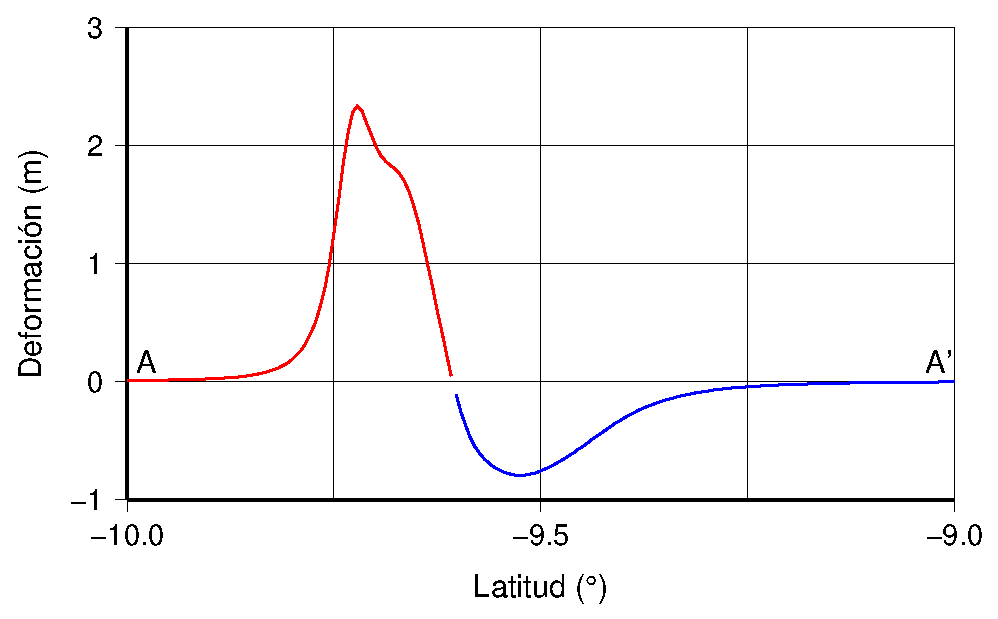
\includegraphics[scale=0.64]{images/figura.eps}}
	\caption{Ejemplo de Figura (en formato eps Encapsulated Post Script).}
	\label{figura1}
\end{figure}

\section{Conclusiones}
Aqui van las conclusiones

De acuerdo a la Figura \ref{figura1}, los valores maximo y minimo son 2.5 y -0.8.

\section*{Agradecimientos}
Aqui van los agradecimientos. Primero se agradece a las personas y luego a las instituciones.


\begin{thebibliography}{99}
	\bibitem[Ape18]{Ape2018} Apellido, N. (2018). Ejemplo de Artículo en Formato APA.\@ \emph{Rev. Inv. Fis., 21} (1), pp 18\textendash26.
	\bibitem[Ben18]{Ben2018} Benny, H. y Pérez, J. (2018). \emph{Título de Libro en Formato APA}. Lima: Editorial San Marcos.
	\bibitem[Kik03]{Kik2003} Kikuchi, M. and Kanamori, H. (2003) Notes on Teleseismic Body\-Wave Inversion Program, web: \url{http://www.eri.u-tokyo.ac.jp/ETAL/KIKUCHI} % chktex 8
	\bibitem[Oco06]{Oco2006} Ocola, L. y Huaco, P. (2006). El maremoto de Chimbote del 21 de febrero de 1996: observaciones de campo. Informe Técnico, Instituto Geofísico del Perú.
	\bibitem[Udi14]{Udi2014} Udías, A., Madariaga, R. y Buforn, E. (2014). Source Mechanism of Earthquakes: Theory and Practice. Cambridge University Press, pp 302.

\end{thebibliography}

\end{document}
